\chapter{Introductory chapter (draft)}

\vspace{0.5cm}

People have wondered for centuries how to improve languages in order to be more efficient, to communicate in an easier way, and with fewer ambiguities.
Most of the time, these questions surface when discussing how to disseminate information and research, notably in scientific fields, when a shared language
between two parties does not exist and a "lingua franca" is required. Thus started the search for an "universal" language.

\section{Universal language}

This line of inquiry is indeed far from being modern: for centuries, Jewish and Catholic scholars searched for the "Adamic language", under the belief that
all of humanity spoke the same language until the construction of the Tower of Babel and the fragmentation of human languages (an event called "confusio linguarum",
the confusion of tongues \footnote{Genesis 11:1-9}). In the seventeenth century, with the sharp decline of Latin as a shared language among scholars, a newfound interest in
the subject sparked since collaboration between researchers of different countries required many of them to become polyglots. While there was an obvious hegemony of the English,
German, and French languages as the "scientific languages" at the time, interest among all research fields in the knowledge originating from countries other than those in Central Europe grew.
Language had become a central factor (or even requirement) to acquire knowledge from authors across the world, and an "universal" language was becoming increasingly important to some.\newline

While discussing the various requirements needed to share one's knowledge with others, philosopher Francis Bacon posited in his 1605 book that some languages use what
he calls "characters real", allowing people that do not share a common oral language to understand each other in written form, which should be a goal when creating a
medium allowing researchers in the fields of science, philosophy and others to communicate:

\begin{quote}
    "(...) And we understand further, that it is the use of China and the kingdoms of the High Levant to write in characters real, which express neither letters nor words in gross, but
    things or notions; insomuch as countries and provinces which understand not one another’s language can nevertheless read one another’s writings, because the characters are accepted
    more generally than the languages do extend; and, therefore, they have a vast multitude of characters, as many, I suppose, as radical words."
    \footnote{\cite{bacon1605proficience} (the position of the quote depends on the various editions and publishing formats of the book, but most commonly found in Book II, Chapter XVI)}
\end{quote}

Other authors explored the same concept, most notably Leibniz and his "characteristica universalis", which according to him allowed users to express mathematical, scientific, and metaphysical
concepts. He wrote at length about it, creating a trove of pictograms and diagrams expressing complex notions (an example of which can be found in
"Dissertatio de arte combinatoria" \footnote{\cite{leibniz1666dissertatio}}).

\begin{figure}[H]
\centering
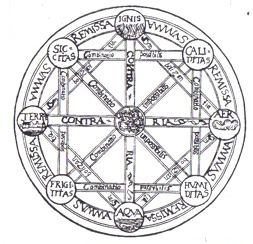
\includegraphics[scale=0.9]{images/characteristica_universalis_diagram.jpg}
\caption{Leibniz's diagrammatic reasoning in "Dissertatio de arte combinatoria"}
\end{figure}

\newpage
While these first forays into the subject solely wanted a language for scholars, more ambitious plans for an artificial language that all nations and people could use came soon after,
with scepticism from several authors. An example of such disagreement can be found in some of Descartes' letters exchanged with fellow polymath Marin Mersenne (in 1629), the former
stating that he does not see any use for such a language, but if it were to exist it would require several aspects:

\begin{itemize}
    \setlength\itemsep{-0.5em}
    \item be international;
    \item outlined by a simple grammar, that could be learned in a few hours;
    \item possess neither exceptions nor irregularities. \footnote{\cite[76-82]{descartes1897oeuvres}}
\end{itemize}

The disagreement notwithstanding, Mersenne eventually created his own "universal language for research", that he presented in his 1636 book
"Harmonie universelle, contenant la th{\'e}orie et la pratique de la musique", containing a proposal for a "perfect language", expressing scientific
concepts through music. \footnote{\cite[Book I, proposition 24]{mersenne1636}}

\section{Constructed languages}

The criteria defined by Descartes are still today the baseline that a lot of authors use for the definition of what an optimal language should be, and are at the core of many
constructed languages. These languages are the artificial counterpart to natural languages: while the latter are the the unconscious natural evolution of existing languages through
time, the grammar, vocabulary, writing system, and other linguistic elements of constructed languages were fully devised from scratch by one or more people. Important note
however --- through use, these constructed languages can also potentially evolve with time, but it is a conscious effort brought forth by its users, and not the effect of human
trends in the language.\newline

Constructed languages are usually divided into three groups, based on their purpose:\newline

\newpage
\textbf{Auxiliary languages}: this group of languages aims to serve as a secondary language for people all around the world to communicate seamlessly.
They serve as a sort of "lingua franca", but without the usual factor of dominance associated to them (socio-economic or political). Some of them have a secondary social aim:
bridge cultures and countries in order to bring peace to the world. Notable examples of languages in this category are Esperanto, Volapük, Ido, and Interlingua.\newline

\textbf{Artistic languages}: group of languages designed as artistic projects, or ways to expand works of fiction and give them more depth. Notable examples of languages
in this category come from many different mediums, such as books (Sindarin and Quenya --- Lord of the Rings, Newspeak --- Nineteen Eighty-Four, and  Nadsat --- A Clockwork Orange),
TV shows (Klingon --- Star Trek, Valyrian and Dothraki --- Game of Thrones, and Goa'uld --- Stargate) or even comic books (Syldavian --- Tintin).\newline

\textbf{Engineered languages}: languages created in order to explore theories in the field of linguistics. Notable examples of languages in this category are Loglan, Lojban, and Toki Pona\newline

A second method of classification for constructed languages was devised in 1903 by Louis Couturat and Léopold Leau in "Histoire de la langue universelle":

\begin{itemize}
    \setlength\itemsep{-0.5em}
    \item A priori system: language whose features are not based on an existing language --- often introducing brand new writing systems, invented grammar structures,
    or a taxonomy for words and concepts;
    \item A posteriori system: language whose features are based in one or several existing languages --- many of which are often criticized for being ethnocentric, and
    creating auxiliary languages that draw inspiration from mostly European countries, which defeats the purpose of an all encompassing world-wide language;
    \item Mixed system: when the language has features that fall into both systems. \footnote{\cite[Introduction, Pages XXVII and XXVIII]{couturat1903histoire}}
\end{itemize}

\newpage
All these classifications are of course loose definitions: a language may fall under more than one category in terms of purpose, for example. For an in-depth history of
constructed languages, I recommend the reader to explore Arika Okrent's book \footnote{\cite{okrent2009land}}. While it is not a scientific publication, it is an extremely
comprehensive and rich book to dive deep into the subject.\newline

\vspace{-0.05cm}
Albeit still being a niche subject, these languages have grown in popularity in the last few years. Following Esperanto, a few of them have risen to the eyes of the public
given their origins. Most of these languages could be classified in the "artistic languages" group, as they originate from works of fiction. Due to the popularity of those works of
fiction, the general public is being exposed to the concept of constructed languages. The most notable example of this growth in popularity is the language learning platform
"Duolingo" introducing courses for three of them: Esperanto, High Valyrian (invented for the TV show "Game of Thrones") and Klingon (invented for the TV show "Star Trek"). \newline

\vspace{-0.05cm}
Unfortunately, due to the notable difference in popularity between Esperanto and other such languages, research in the field of linguistics has mostly been focused on the former.
This focus is understandable: Esperanto is one of the few constructed languages that can boast having native speakers. Detlev Blanke highlights this achievement, putting Esperanto
in a category of its own as a full-fledged language, and not a "language project" or a "semilanguage". He theorises that it is the only constructed language that has gone through nineteen
evolutionary steps he describes, "from the publication of its structure to the appearance of the first bilingual children" \footnote{\cite{blanke1989planned}}.
Since the publication of his article, Klingon can probably claim the same status, but researchers probably don't delve into it as much due to its origins.
Nonetheless, authors have been urging researchers to study other constructed languages, as these may have troves of interesting linguistic elements \footnote{\cite{oostendorp2001constructed}}.

\section{Lojban}

\subsection{The roots: the history of Loglan}

The first constructed language whose main aim is optimality is most probably Loglan, introduced by James Cooke Brown and first published
in Scientific American \footnote{\cite{brown1960loglan}}. This is a notable achievement: rarely had a major scientific periodical devoted publishing
space to a constructed language other than Esperanto. This is probably due to the fact that Brown presented it with a purely scientific approach, and no big societal aims
(at first --- history will change that). Loglan, whose name is a contraction of the words "Logical" and "Language", was defined as having the following aims:

\begin{itemize}
    \setlength\itemsep{-0.5em}
    \item be purely based in logic;
    \item be culturally neutral;
    \item have a grammar small enough to be teachable, but complex enough to allow conversations;
    \item be unambiguous.
 \end{itemize}

The history of Loglan will take a strange path after its first publication. Given its publication in a major scientific journal, and a growing audience
asking him for more information, Brown requested a raise from his university, which was declined, and a government grant, which was also refused multiple times.
Insulted, he eventually resigned from his research position and, using money gathered by activities other than scientific research, started his own institute,
the "Loglan Institute". Later, in 1975, he published a book about the language. At the institute, he surrounded himself mostly by admirers, most of which were computer science
students and researchers who were excited by the possibility of the language serving as a human-computer interface. Thus, Brown rarely opened himself to critics,
which might have influenced the inflated sense of importance he felt Loglan had. A less explicit aim for the language, that was presented at a later point, was attempting
to prove the hypothesis of linguistic relativity (also known as the Sapir–Whorf hypothesis, or simply the Whorf hypothesis) in its strong version.
Most modern linguists would disagree with this statement, but Brown was convinced that the usage of Loglan would allow speakers to think more logically, and expand their
intelligence.\newline

With a growing audience, and the transformation of the institution into a "membership-controlled corporation" (in order to request paying fees to all the volunteers),
Brown started to see that its members wanted to steer his creation in a direction he did not enjoy. Trying to remain in control, he fired most of the board.
This event and others created a schism in the Loglan community, and little by little a separatist group grew, which gave birth to Lojban.

\subsection{The creation of Lojban}

Starting in 1987, The Logical Language Group (LLG) worked to create a constructed language that aimed to extend the existing Loglan language and improve it further,
in order to make it easier to learn by humans and more readily accessible. This work culminated with the publication of a book in 1997 by
John Woldemar Conwan \footnote{\cite{cowan1997complete}}, an American programmer otherwise known for his work with XML and Unicode, among other things. This book is,
still today, considered the baseline of the language, defining its whole grammar, vocabulary, and semantics.\newline

Over the years, Brown disputed several times in court that this creation infringed his copyright. Several trials later, all courts agree that both projects are independent,
and Lojban took over Loglan in popularity and contributors.

\subsection{Brief introduction to the Lojban grammar}

Lojban sentences are constructed in a way that expresses a logical predicate, with a fixed set of arguments. For a small
refresher course in predicate logic see Annex A. The recurring "first approach to the language" example used in most Lojban
literature, from the language standard to research papers is the sentence "John is the father of Sam". In this sentence, there
is a clear predicate ("is-the-father-of") and two arguments ("John" and "Sam").

\begin{figure}[H]
\centering
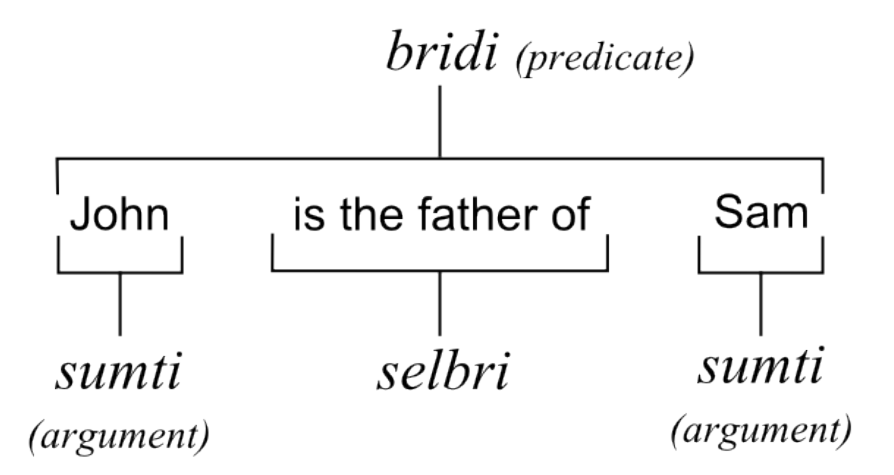
\includegraphics[scale=0.20]{images/lojban_grammar.png}
\caption{Basic structure of a Lojban sentence (Source: \cite{cowan1997complete})}
\end{figure}

This figure presents the three most important base elements of a sentence in Lojban:

\begin{itemize}
    \item \textbf{bridi}: the predicate expression;
    \item \textbf{selbri}: the word(s) acting as the predicate;
    \item \textbf{sumti}: positional argument passed to the predicate.
\end{itemize}

Selbri are strictly defined by representations which position the sumti around a key word. For example, the selbri to describe the fatherhood relationship is "patfu":

$$\text{patfu}: x_1 \: \text{is a father of} \: x_2$$

Thus, the above sentence is expressed in Lojban as: \textbf{la .djon. patfu la .sam.} \newline

If no modifiers are used, the position of the sumti is rigid and allows to release the sentence from any ambiguity. We always know who is the father and who is the child.
Of course, in this example, the English counterpart doesn't really make sense (the sentence "Sam is 'fathered' by John" makes absolutely no sense), but for a non-native speaker
the order of words in other pairs of sentences might add ambiguity. For example, a non-native might get confused about the difference between the sentences
"My dog bites the man" (\textbf{"le mi gerku cu batci le nanmu"} in Lojban) and "The man is being bitten by my dog", as this inverted construct might not exist in their language.
Lojban solves this issue by having a specific keyword, indicating that two or more sumti (positional arguments) are going to be swapped. This allows speakers, even those not
familiar with this grammatical construct, to understand the difference between two very different sentence constructions: e.g. "The man is being bitten by my dog"
and "The man is biting my dog".\newline

Of course, this framework of predicate expressions is simply the base feature of the language, but many others allow it to cover the other missing aspects that most natural
languages feature: tenses, relative clauses, abstractions, emotional indicators, and many others. These will be explored in a further chapter of the thesis. \newline

\section{What this thesis aims to achieve}

At its root, computer science had a singular aim --- automating calculations for a broad spectrum of use-cases. However with time and with the emergence of better, faster, and
stronger computers, researchers understood that computers could be used to achieve far more complex tasks. Several diverse research fields made their appearance, and among these
some realised that computing could help us structure the flow of information, in addition to making calculations based on it. \newline

The explosion of tasks requiring the processing of large amounts of structured data inside of companies, and much later the arrival of the Internet, forced us to debate and
research subjects such as: how to gather information, how to manage and store it, analyse and interpret it, explore it, etc... A sizeable chunk of this information comes to us
in the form of text and language, in their many forms. To answer these needs, language engineering became a central research field in a new society, one that had migrated
from a purely industrial society to an "information society".\newline

The main aim of this thesis is to explore the intersection between the two fields presented in this introduction: linguistics, around the subject of a particular constructed
language, and computer science, which allows language processing. The first objective of this thesis is to outline the state of the art and existing parsers for Lojban, list both
their flaws and positive aspects, and define what kind of new parser would be interesting to develop. Using the Python programming language, one such parser will be created, including
also a way to visualise the structure of the sentences parsed, in order to analyse them.\newline

A second objective is to create a minimal proof of concept of machine translation using Lojban as an interlingua between English and French --- if that turns out to be possible.
This type of translation method would of course never challenge existing models, which are based on artificial intelligence and have shown incredible results that never cease to
improve. However, it is an interesting research prototype: Lojban claims to be a syntactically unambiguous language that improves human-human communication but also human-computer
communication. While the former is more complicated to prove, since the amount of speakers of Lojban around the world is not immense, the latter has been studied. Research has already
postulated that Lojban (or variants of it) would be interesting interlinguas between humans and computers \footnote{\cite{speer2004meeting}} or artificial
intelligences \footnote{\cite{goertzel2013lojban}}.
